\documentclass[]{article}
\usepackage{lmodern}
\usepackage{amssymb,amsmath}
\usepackage{ifxetex,ifluatex}
\usepackage{fixltx2e} % provides \textsubscript
\ifnum 0\ifxetex 1\fi\ifluatex 1\fi=0 % if pdftex
  \usepackage[T1]{fontenc}
  \usepackage[utf8]{inputenc}
\else % if luatex or xelatex
  \ifxetex
    \usepackage{mathspec}
    \usepackage{xltxtra,xunicode}
  \else
    \usepackage{fontspec}
  \fi
  \defaultfontfeatures{Mapping=tex-text,Scale=MatchLowercase}
  \newcommand{\euro}{€}
\fi
% use upquote if available, for straight quotes in verbatim environments
\IfFileExists{upquote.sty}{\usepackage{upquote}}{}
% use microtype if available
\IfFileExists{microtype.sty}{%
\usepackage{microtype}
\UseMicrotypeSet[protrusion]{basicmath} % disable protrusion for tt fonts
}{}
\usepackage[margin=1in]{geometry}
\usepackage{graphicx}
\makeatletter
\def\maxwidth{\ifdim\Gin@nat@width>\linewidth\linewidth\else\Gin@nat@width\fi}
\def\maxheight{\ifdim\Gin@nat@height>\textheight\textheight\else\Gin@nat@height\fi}
\makeatother
% Scale images if necessary, so that they will not overflow the page
% margins by default, and it is still possible to overwrite the defaults
% using explicit options in \includegraphics[width, height, ...]{}
\setkeys{Gin}{width=\maxwidth,height=\maxheight,keepaspectratio}
\ifxetex
  \usepackage[setpagesize=false, % page size defined by xetex
              unicode=false, % unicode breaks when used with xetex
              xetex]{hyperref}
\else
  \usepackage[unicode=true]{hyperref}
\fi
\hypersetup{breaklinks=true,
            bookmarks=true,
            pdfauthor={Kushal K Dey},
            pdftitle={Topic model with Batch effects},
            colorlinks=true,
            citecolor=blue,
            urlcolor=blue,
            linkcolor=magenta,
            pdfborder={0 0 0}}
\urlstyle{same}  % don't use monospace font for urls
\setlength{\parindent}{0pt}
\setlength{\parskip}{6pt plus 2pt minus 1pt}
\setlength{\emergencystretch}{3em}  % prevent overfull lines
\setcounter{secnumdepth}{0}

%%% Use protect on footnotes to avoid problems with footnotes in titles
\let\rmarkdownfootnote\footnote%
\def\footnote{\protect\rmarkdownfootnote}

%%% Change title format to be more compact
\usepackage{titling}

% Create subtitle command for use in maketitle
\newcommand{\subtitle}[1]{
  \posttitle{
    \begin{center}\large#1\end{center}
    }
}

\setlength{\droptitle}{-2em}
  \title{Topic model with Batch effects}
  \pretitle{\vspace{\droptitle}\centering\huge}
  \posttitle{\par}
  \author{Kushal K Dey}
  \preauthor{\centering\large\emph}
  \postauthor{\par}
  \predate{\centering\large\emph}
  \postdate{\par}
  \date{January 22, 2016}



\begin{document}

\maketitle


\subsection{Introduction}\label{introduction}

In RNA-seq experiments, we often encounter samples coming from different
batches. The batches may be determined by the different amplification
procedures, sequencing machines or even sequencing lanes used for
sequencing. When such effects are present in the samples, it becomes
difficult to separate out the biological effects from the technical
effects (the latter is often relatively stronger). The topic model or
the grade-of membership model has been used to cluster the samples based
on their RNA-seq reads counts data (see
\href{https://github.com/stephenslab/count-clustering/blob/master/docs/main.pdf}{paper}).
In the paper, we have shown that the topic model is sensitive to the
presence of batch effects, however we have not been able to present a
solution to that problem. Here, we try to address the issue of how one
can tackle batch effects in a topic model type framework.

We first present the standard topic model framework

\subsection{Standard Topic Model}\label{standard-topic-model}

Let \(c_{ng}\) be the counts of reads for sample \(n\) and gene \(g\).
Let \(c_{n+}\) be the sum of reads for sample \(n\), also called the
\emph{library size}.

\[ (c_{n1}, c_{n2}, \cdots, c_{nG}) \sim Mult (c_{n+}, p_{n1}, p_{n2}, \cdots, p_{nG})  \]

\[ p_{ng} = \sum_{k=1}^{K} \omega_{nk} \theta_{kg} \hspace{1 cm} \sum_{k} \omega_{nk} =1 \hspace{0.5 cm} \forall n \hspace{1 cm} \sum_{g} \theta_{kg} =1 \hspace{0.5 cm} \forall k\]

Here \(\omega_{n.}\) represents the topic proportions for \(n\) th
samples. On the other hand \(\theta_{k.}\) represents the probability
distribution on the genes for the \(k\)th topic or cluster.

\subsection{Topic model with Batch
effects}\label{topic-model-with-batch-effects}

One way batch effects may be incorporated in the above model would be to
make the topic distribution for each cluster/ topic a function of the
batch the sample is coming from. Then we can write the above model as

\begin{equation}
(c_{n1}, c_{n2}, \cdots, c_{nG}) \sim Mult (c_{n+}, p_{n1}, p_{n2}, \cdots, p_{nG})
\label{lab:mult}
\end{equation}

\begin{equation}
p_{ng} = \sum_{k=1}^{K} \omega_{nk} \theta_{b(n):k,g} \hspace{1 cm} \sum_{k} \omega_{nk} =1 \hspace{0.5 cm} \forall n \hspace{1 cm} \sum_{g} \theta_{b(n):k,g} =1 \hspace{0.5 cm} \forall k, \hspace{0.5 cm} b(n) \in \{1,2,\cdots, B \}
\end{equation}

\subsection{Prior Specification}\label{prior-specification}

Note that the above the model is analogous to applying topic model
separately for each batch. The problem with that approach is that we
will not be able to track which biological cluster in Batch 1
corresponds to which biological cluster in Batch 2. We expect each
cluster distribution to have some common features across different
batches despite getting effected by batch effects and we want to account
for that similarity in patterns. In order to do that, we assume for each
cluster \(k\)

\begin{equation}
(\theta_{b:k, 1}, \theta_{b:k, 2}, \cdots, \theta_{b:k, G}) \sim Dir_{G} \left ( \theta_{k1}, \theta_{k2}, \cdots, \theta_{kG} \right ) \hspace{1 cm} b \in \{1,2, \cdots, B \} 
\label{lab:prior}
\end{equation}

which is same as saying that for each batch, we are generating a sample
from the cluster with mean
\((\theta_{k1}, \theta_{k2}, \cdots, \theta_{kG})\), representing the
cluster \(k\).

The above specification is analogous to the assumptions in normal linear
models with batch effects,

\[ y_{nl} = \mu_{t(n):b(n),l} + e_{nl} = \mu + \tau_{t(n)} + \beta_{b(n)} + e_{nl} \hspace{0.5 cm} e_{nl} \sim N(0,\sigma^2_{e}) \]

where \(t(n)\) in the treatment effect and \(b(n)\) is the batch effect.
We often assume that

\[ \beta_{b} \sim N(0, \sigma^{2}_{b}) \hspace{1 cm} b \in \{1,2, \cdots, B \} \]

Then

\[ \mu_{t(n):b(n),l} \sim N (\mu + \tau_{t(n)}, \sigma^{2}_{e})  : = N(\mu_{t(n)}, \sigma^{2}_{e}) \hspace{0.5 cm} \forall l\]

Notice that the treatment effects under different batches are a random
sample from a distribution whose mean is the overall treatment effect.
Note that \(\sigma_b\) term is the tuning parameter for each batch, that
takes into account the inherent variability in a batch. We can also put
such a scaling parameter in our model Equation \ref{lab:prior}.

Then for each \(k\),

\[ (\theta_{b:k, 1}, \theta_{b:k, 2}, \cdots, \theta_{b:k, G}) \sim Dir_{G} \left ( \alpha_{b} \theta_{k1}, \alpha_{b} \theta_{k2}, \cdots, \alpha_{b} \theta_{kG} \right ) \hspace{1 cm} b \in \{1,2, \cdots, B \} \]

However, as of now, I am assuming that \(\alpha_b =1\) for all batches
and working with the simpler model.

We assume a prior for \(\theta_{kg}\).

\begin{equation}
(\theta_{k1}, \theta_{k2}, \cdots, \theta_{kG}) \sim Dir_{G} \left ( \frac{1}{KG}, \frac{1}{KG}, \cdots, \frac{1}{KG} \right) \hspace{1 cm} \forall k
\label{lab:prior2}
\end{equation}

So, essentially we have a hierarchical structure in the \(\theta\)'s, on
combining Equation \ref{lab:prior} and Equation \ref{lab:prior2}.

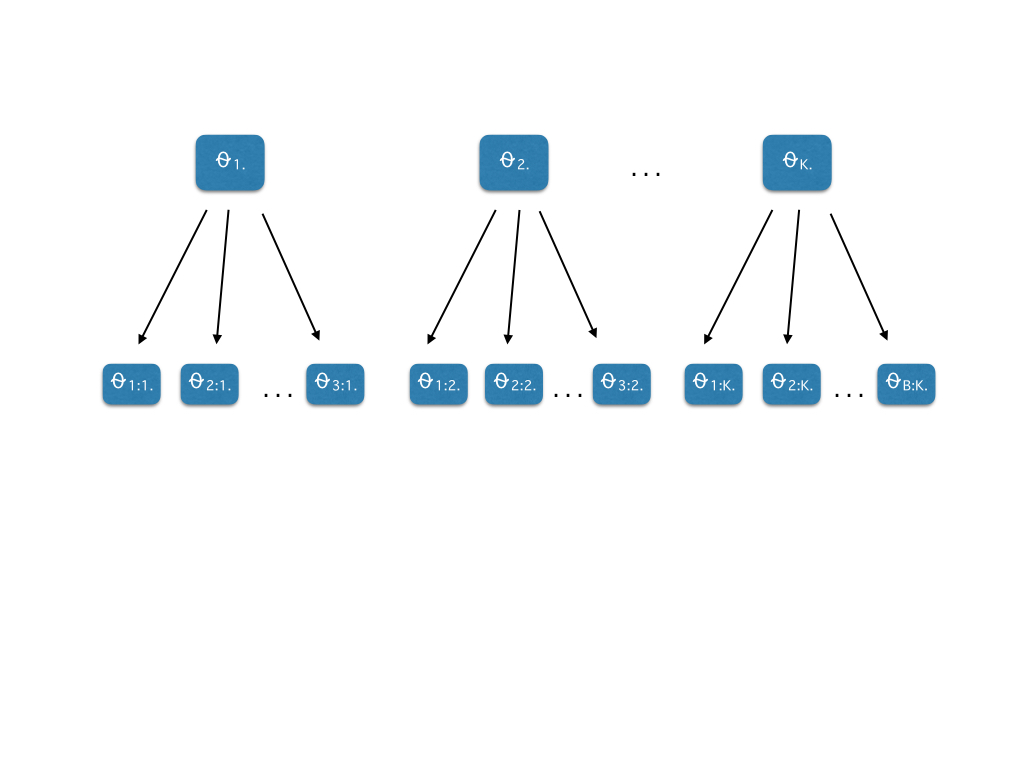
\includegraphics{../figs/hierarchy_batch.jpeg} We can assume the same
prior for \(\omega\) as in standard topic model, given by

\[ (\omega_{n1}, \omega_{n2}, \cdots, \omega_{nK}) \sim  Dir_{K} \left ( \frac{1}{K}, \frac{1}{K}, \cdots, \frac{1}{K} \right) \hspace{1 cm} \forall n\]

\subsection{Model Specifications}\label{model-specifications}

We can assume that

\begin{equation}
c_{n+} \sim Poi(\lambda_{n}) 
\label{lab:libsize}
\end{equation}

Combining Equation \ref{lab:mult} and Equation \ref{lab:libsize}, we get

\begin{equation}
c_{ng} \sim Poi \left ( \lambda_{n} \sum_{k} \omega_{nk} \theta_{kg} \right)
\end{equation}

Let \(z_{nkg}\) represents the number of counts from sample \(n\) and
gene \(g\) that comes from \(k\) th subgroup or cluster. By definition,

\[ \sum_{k=1}^{K} z_{nkg} = c_{ng}  \]

Since the summation of two independent Poisson random variables is also
a Poisson variable with mean equal to the sum of the means of the
original random variables, we can infer that

\[ z_{nkg} \sim Poi \left (\lambda_{n}\omega_{nk} \theta_{b(n):k,g} \right ) \]

Let \(z_{bkg}\) be the latent variable representing the number of reads
coming from the \(b\) th batch, \(k\) th subgroup/ cluster and gene
\(g\).

\[ z_{bkg} | \theta_{b:k,g} \sim Poi \left (\theta_{b:k,g} \sum_{b(n):b} \omega_{nk}\lambda_{n} \right )  \]

\[ z_{kg} | \theta_{b:k,g} \sim Poi \left (\sum_{b} \theta_{b:k,g} \sum_{b(n):b} \omega_{nk}\lambda_{n} \right ) \]

We can write

\begin{align*}
E(z_{kg} | \theta_{kg}) & = E \left ( \sum_{b} E \left ( z_{bkg} | \theta_{b:k,g} \right)| \theta_{kg} \right ) \\
                        & = E \left ( \sum_{b} \theta_{b:k,g} \sum_{b(n):b} \omega_{nk} \lambda_{n} |  \theta_{kg} \right) \\
                        & = \theta_{kg} \sum_{n} \omega_{nk} \lambda_{n} 
\end{align*}

However despite a simple looking expression for the expectation, the
distribution of \(z_{bkg}\) or \(z_{kg}\) given \(\theta_{kg}\) is
pretty complicated.

\begin{equation}
z_{bkg} | \theta_{kg} \sim \prod_{b=1}^{B} \frac{\Gamma (\sum_{g} \theta_{kg})}{\Gamma (\sum_{g} z_{bkg} + \sum_{g} \theta_{kg})} \prod_{g=1}^{G} \frac{\Gamma (z_{bkg} + \theta_{kg})}{\Gamma (\theta_{kg})} \theta^{1/KG}_{kg} 
\label{lab:distr1}
\end{equation}

and

\begin{equation}
z_{kg} = \sum_{b} z_{bkg}
\label{lab:distr2}
\end{equation}

This density is difficult to handle and will be time expensive to solve
for \(\theta\) using this density function. Therefore, we resort to a
more simplified approach, through EM algorithm type mechanism to obtain
parameter updates at each step.

\subsection{Model Estimation}\label{model-estimation}

Suppose at the end of update \(n\), the current estimates we have are
\(\omega^{(m)}_{nk}\), \(\theta^{(m)}_{b:k,g}\) and
\(\theta^{(m)}_{kg}\). We use these iterates to obtain refined estimates
\(\omega^{(m+1)}_{nk}\), \(\theta^{(m+1)}_{b:k,g}\) and
\(\theta^{(m+1)}_{kg}\). We first update the \(\theta^{(m+1)}_{b:k,g}\)
given the known parameter values using EM algorithm.

\begin{equation}
\mathcal{L} (z_{bkg} | \theta_{b:k,g}) := Poi \left (\theta_{b:k,g} \sum_{b(n):b} \omega_{nk}\lambda_{n} \right )  
\label{lab:loglik}
\end{equation}

or

\begin{equation}
\mathcal{L} (z_{bk1}, z_{bk2}, \cdots, z_{bkG} | \theta_{b:k,.}) := Mult \left (z_{bk+}, \theta_{b:k,1}, \theta_{b:k,2}, \cdots, \theta_{b:k,G} \right)
\label{lab:loglik}
\end{equation}

\begin{equation}
\pi(\theta_{b:k,.} | \theta_{k.} ) \propto \prod_{g=1}^{G} \theta_{b:k,g}^{\theta_{kg}}
\label{lab:prior}
\end{equation}

We define the E-step of the EM algorithm as follows (done separately for
each \(k\))

\begin{equation}
\mathcal{Q} \left ( \theta_{b:k,.} | C_{N \times G}, \theta^{(m)}_{b:k,.}, \theta^{(m)}_{k.} , \omega^{(m)} \right ) = \mathbb{E}_{Z | C_{N \times G}, \theta^{(m)}_{b:k,.}, \theta^{(m)}_{k.} , \omega^{(m)}} \left ( log \; \mathcal{L} (z_{bk1}, z_{bk2}, \cdots, z_{bkG} | \theta_{b:k,.})  + log \; \pi(\theta_{b:k,.} | \theta^{(m)}_{k.} ) \right )
\label{lab:estep}
\end{equation}

We next perform the M-step and we obtain the following solutions for
\(\theta_{b:k,g}\)s.

\begin{equation}
\theta^{(m+1)}_{b:k,g} : = \frac{\mathbb{E} \left ( z_{b:k,g} |  C_{N \times G}, \theta^{(m)}_{k.} , \omega^{(m)} \right) + \theta^{(m)}_{kg}}{\sum_{g} \mathbb{E} \left ( z_{b:k,g} |  C_{N \times G}, \theta^{(m)}_{k.} , \omega^{(m)} \right) + 1}
\label{lab:mstep}
\end{equation}

The expectation over
\([ z_{b:k,g} | C_{N \times G}, \theta^{(m)}_{b:k,.}, \theta^{(m)}_{k.} , \omega^{(m)} ]\)
is given by the following

\[ \mathbb{E} \left ( z_{b:k,g} |  C_{N \times G}, \theta^{(m)}_{b:k,.}, \theta^{(m)}_{k.} , \omega^{(m)} \right) : = c_{ng} \frac{\omega^{(m)}_{nk} \theta^{(m)}_{b:k,g}}{\sum_{h=1}^{K} \omega^{(m)}_{nh} \theta^{(m)}_{b:h,g}} \]

Once we obtain the estimates \(\theta^{(m+1)}_{b:k,g}\), then we would
like to update \(\theta^{(m+1)}_{kg}\) conditional on
\(\theta^{(m+1)}_{b:k,g}\) for all \(b \in \{1,2, \cdots, B \}\).

One can assume \(\theta^{(m+1)}_{b:k,.}\) for all \(b\) to be a random
sample of size \(B\) (same as number of batches) given \(\theta_{k.}\)
and given the data, we want to estimate the parameters \(\theta_{k.}\).
However estimating MLE of the Dirichlet parameters is not easy
(specially with so many parameters-G is usually pretty big), and
requires Newton-Raphson Method (check
\href{http://www.msr-waypoint.com/en-us/um/people/minka/papers/dirichlet/minka-dirichlet.pdf}{paper}).
One can obtain a MOM (Methods of Moments) type estimator with a tuning
parameter \(\nu\) as follows.

\[ \theta^{(m+1)}_{kg} = \frac{1}{B+\nu} \sum_{b=1}^{B} \theta^{(m+1)}_{b:k,g}  + \frac{\nu}{B+\nu} \frac{1}{G} \]

instead of the MLE estimator derived from the conditional distribution
of \(z_{kg}\) given \(\theta_{kg}\) as given in Equation
\ref{lab:distr1} and Equation \ref{lab:distr2}. However as discussed
earlier, the original conditional distribution of
\(z_{kg} | \theta_{kg}\) seems difficult to handle.

We fix the batch \(b\). Then given \(\theta^{(m+1)}_{b:k,g}\), we can
estimate \(\omega^{(m+1)}_{nk}\) from \(\omega^{(m)}_{nk}\) and
\(\theta^{(m+1)}_{b:k,g}\) using similar convex optimization technique
used by Matt Taddy in his
\href{http://arxiv.org/pdf/1109.4518v3.pdf}{paper}.

At the end of these steps, we will have \(\omega^{(m+1)}_{nk}\),
\(\theta^{(m+1)}_{b(n):k,g}\) and \(\theta^{(m+1)}_{kg}\). We can these
use these to update the parameters further and we continue till the
log-likelihood converges.

\end{document}
